\documentclass[12pt]{book}
\usepackage[margin=2cm, bindingoffset=0cm]{geometry}
%\usepackage[german]{babel} 
\usepackage[ngerman]{babel} %sudo apt-get install texlive-lang-german
\usepackage{hyperref} % web links etc.
\usepackage[parfill]{parskip}
\usepackage[utf8]{inputenc}
\usepackage[dvipsnames]{xcolor}
\usepackage{tcolorbox}
\usepackage{helvet} 
\usepackage{framed}
\usepackage{anyfontsize}
\usepackage{csquotes}
\usepackage{physics}
\usepackage{amssymb}
\MakeOuterQuote{"}
\definecolor{quotecolor}{rgb}{0.8,0.9,1}
\renewcommand{\familydefault}{\sfdefault} 
\setlength\parindent{0pt}
\tcbset{
  boxrule=0pt,
  colback=quotecolor,
  arc=5pt,
  auto outer arc,
  left=5pt,
  right=5pt,
  boxsep=5pt
}
%  width=0.9\textwidth,

\begin{document}
\title{\fontsize{40}{40}\selectfont \textbf{Die Schrift}}
\date{\today}
\maketitle

\chapter{Wozu diese Schrift?}

Diese Schrift soll dich verändern. Jede Schrift, die du liest, verändert dich. 
Ich will, dass diese Schrift dein Denken in eine bestimmte Richtung verändert.
Diese Schrift ist nicht dazu da, mir zum Broterwerb zu dienen.
Es geht einzig und allein darum, dich zu verändern. Von solcher Art ist diese Schrift. 

Wenn du meinst, dass du dich nicht ändern solltest, zum Beispiel weil du dich
bereits perfekt findest, dann kehre jetzt um und lies nicht weiter!

\section{Warum will ich dein Denken ändern?}

Die kurze Antwort ist: aus Mitleid. 

Wenn du meinst, dass du kein Mitleid benötigst, dann warte ab und 
schaue, was dir das Leben bringen wird! Und danach komme wieder, falls du noch kannst!

Die lange Antwort ist: Du wirst sterben. Du wirst leiden. Du wirst nicht verstehen, warum du leiden musst.
Während du lebst, wirst du Vielen unnötiges Leid zufügen. Das wirst du teilweise absichtlich machen, viel öfter 
wirst du es aber unabsichtlich machen. Diese Schrift soll dir helfen zu erkennen, dass du
weder deinem eigenen Leiden noch dem Leidzufügen aus dem Wege gehen kannst.
Das ist einem Menschen nicht möglich. Dennoch kannst du versuchen, diese Leiden zu verringern.

Vielleicht gehörst du zu den unglücklichen Tröpfen, die sich ständig um das Morgen sorgen.
Ich sage dir: du brauchst dich nicht sorgen, denn morgen kannst du schon tot sein. Vielleicht sogar heute schon.

Oder haderst du mit der Welt? Geht sie in eine schlechte Richtung?
Ich sage dir: weder kannst du wissen, was gut oder schlecht ist, noch in welche Richtung sie gehen wird.
Du kannst nicht mal wissen, ob sie überhaupt geht. Vielleicht bist nur du es, der geht.

Hast du vielleicht Angst vor dem Tod? Du sollst verstehen, warum du diese Angst hast.
Doch vielleicht weißt du nicht, was der Tod ist. Vielleicht weißt du nicht mal, was Leben ist?

\section{In welche Richtung will ich dein Denken ändern?}

Dies ist eine philosophische Schrift. Es geht um Erkenntnis. Wenn du als naiver Realist hier aufschlägst, soll diese Schrift
dein Denken dramatisch umdrehen. Niemals würdest du dich als naiv bezeichnen?

Wenn du diese Sätze verstehst, dann bist du kein naiver Realist mehr, und diese Schrift kann dir nicht viel Neues geben:
\begin{quote}\begin{tcolorbox}
Jedes Elementarteilchen enthält alle anderen Elementarteilchen.
\end{tcolorbox}\end{quote}
\begin{quote}\begin{tcolorbox}
There are no particles!
\end{tcolorbox}\end{quote}
\begin{quote}\begin{tcolorbox}
Die Summe zweier Teile ist ihr Produkt. Im Produkt sind die Teile enthalten und nicht enthalten. 
Auch unendlich viele andere 2 Teile sind im Produkt enthalten und nicht enthalten.
\end{tcolorbox}\end{quote}
\begin{quote}\begin{tcolorbox}
Keine Nachricht enthält eine Bedeutung. Auch diese Schrift enthält keine Bedeutung.
\end{tcolorbox}\end{quote}
\begin{quote}\begin{tcolorbox}
Bei diesen kleinsten Lebewesen aber wird die Frage, ob sie aus lebendiger oder toter Materie bestehen, unentscheidbar. Man kann dies so ausdrücken, daß es überhaupt nur lebendige Materie gebe; ...
\end{tcolorbox}\end{quote}
\begin{quote}\begin{tcolorbox}
Eigentlich gibt es gar nichts Unlebendiges! ...
\end{tcolorbox}\end{quote}
\begin{quote}\begin{tcolorbox}
Dass ein Tisch im Grunde auch lebendig ist, bemerken wir nicht, weil wir ihn nur vergröbert betrachten und damit vereinfacht sehen.
\end{tcolorbox}\end{quote}

Wenn du als Materialist hier aufschlägst, sollst du als Idealist wieder herausgehen.

Hinter dieser Schrift steckt der feste Glaube: wenn du mehr erkennst von der Welt und dir selbst,
dann wird sich über kurz oder lang dein Handeln von selbst in die gewollte Richtung ändern. Du wirst weniger wollen, mit weniger zufrieden
oder gar glücklich sein. Du wirst Leid vermeiden wollen. Du wirst dein Handeln von der Liebe leiten lassen, weil du weißt,
dass es sonst nichts gibt, an dem du dich festhalten kannst.

\section{Wie werden wir es tun?}

Wir beginnen mit dem philosophischen Fundament von Descartes.
Wir erkennen die Schleier, die unser Denken vernebeln und uns an der Erkenntnis hindern.
Wir sehen nach, was die Wissenschaft uns seit den alten Zeiten der Philosophie Neues gebracht hat.
Wir gehen die harte Tour, auch mit Mathematik, weil die Sprache der Mathematik näher an der Wahrheit ist als unsere Alltagssprache, welche einer der Schleier ist.

\chapter{Philosophischer Startpunkt}

\section{ego cogito, ergo sum}

\begin{quote}\begin{tcolorbox}
Indem wir so alles nur irgend Zweifelhafte zurückweisen und für falsch gelten lassen, können wir leicht annehmen, dass es keinen Gott, keinen Himmel, keinen Körper gibt; dass wir selbst weder Hände noch Füße, überhaupt keinen Körper haben; aber wir können nicht annehmen, dass wir, die wir solches denken, nichts sind; denn es ist ein Widerspruch, dass das, was denkt, in dem Zeitpunkt, wo es denkt, nicht bestehe. Deshalb ist die Erkenntnis: »Ich denke, also bin ich,« von allen die erste und gewisseste, welche bei einem ordnungsmäßigen Philosophieren hervortritt.
\end{tcolorbox}\end{quote}

Dies war für René Descartes das nicht weiter kritisierbare Fundament der Ontologie, das heißt der Lehre vom Seienden. Wir wissen also sicher

\emph{Etwas erkennt, dass da etwas ist (nämlich wenigstens das Erkennende selbst).}

Dieses Erkennende mag man als \emph{Ich} bezeichnen, ich will es aber lieber als \textbf{Bewusstsein} bezeichnen, also als das, was sich dem Dasein einer Welt bewusst ist. Wir wissen damit sicher, dass Bewusstsein existiert, und darüber hinaus wissen wir nichts. Der hier verwendete Bewusstseinsbegriff hat nichts mit einem Speicher für Erinnerungen oder noch spezieller mit einem Gehirn zu tun. Er ähnelt mehr dem Begriff \emph{Geist}, will aber zusätzlich die reflexive Eigenschaft, die Rückbeziehung des Geistes auf sich, betonen. 

Es ist wichtig, dass du diese erste Erkenntnis von Descartes verstehst und verinnerlichst. Sie ist der allererste Schritt zu weiterer philosophischer Erkenntnis. Arthur Schopenhauer beginnt das 1. Buch seines Hauptwerks \emph{Die Welt als Wille und Vorstellung} hiermit: 

\begin{quote}\begin{tcolorbox}
»Die Welt ist meine Vorstellung:« – dies ist die Wahrheit, welche in Beziehung auf jedes lebende und erkennende Wesen gilt; wiewohl der Mensch allein sie in das reflektirte abstrakte Bewußtseyn bringen kann: und thut er dies wirklich; so ist die philosophische Besonnenheit bei ihm eingetreten. Es wird ihm dann deutlich und gewiß, daß er keine Sonne kennt und keine Erde; sondern immer nur ein Auge, das eine Sonne sieht, eine Hand, die eine Erde fühlt; daß die Welt, welche ihn umgiebt, nur als Vorstellung da ist, d.h. durchweg nur in Beziehung auf ein Anderes, das Vorstellende, welches er selbst ist.
\end{tcolorbox}\end{quote}

Dieser Satz führt zum Teil schon weiter. Mir ist hier nur die Verknüpfung zwischen philosophischer Besonnenheit und dem Anzweifeln der Existenz von Sonne und Erde wichtig. So lange du nicht an deren Existenz zweifelst, so lange bleibst du ein naiver Realist. 

Natürlich bleibt der Zweifel nicht bei Sonne und Erde stehen. Auch die Existenz von Auge und Hand muss angezweifelt werden, nicht aber die des Vorstellenden, welches er selbst ist. \emph{Er} ist aber \emph{nicht der Mensch}, denn auch die Existenz von Menschen muss angezweifelt werden. \emph{Er} ist das Bewusstsein.

\section{Zeit}

Dem Bewussstsein ist Änderung fest eingebaut. Der treffendere Begriff wäre eigentlich Bewusst\emph{werden} und nicht Bewusst\emph{sein}. Aus demselben Grund favorisierten Schopenhauer und Dürr den Begriff \emph{Wirklichkeit}, der ein ständiges Werden ausdrückt, vor dem Begriff \emph{Realität}, der ein dauerhaftes Sein von Dingen ausdrückt. Wir können das Bewusstwerden nicht abschalten. Damit einher geht die Vorstellung einer (seienden) vergehenden Zeit, einer Variable, die unsere Bewusstwerdungen durchnummeriert und ordnet. Wir wollen diese Zeit \textbf{psychische Zeit} nennen.

In der Mechanik von Newton ist diese psychische Zeit universell, schlichtweg "die Zeit". Doch die physikalische Wissenschaft musste, zuerst mit der speziellen Relativitätstheorie, erfahren, dass diese Gleichsetzung nicht aufrecht erhalten werden kann. Wir werden darauf noch zurückkommen.

\section{Kontinuierliche Empfindungen}

Auf das Bewusstsein strömen \emph{kontinuierlich} \textbf{Empfindungen} ein. Dies ist ein ganz wichtiger Punkt: \textbf{Es werden keine Einzeldinge bewusst}. Wenn du nur genau genug hinsiehst, dann musst du zugeben, das sich die Bilder oder Töne oder sonstigen Empfindungen \emph{kontinuierlich} vor dem Bewusstsein wandeln, oder dass das Bewusstwerden ein kontinuierlicher Wandel ist. Diese Erkenntnis ist Jahrtausende alt. Heraklit von Ephesos hat sie so formuliert:

\begin{quote}\begin{tcolorbox}
Alles ist im Fluß.
\end{tcolorbox}\end{quote}

Und Arthur Schopenhauer so:

\begin{quote}\begin{tcolorbox}
... ewiges Werden, endloser Fluß gehört zur Offenbarung des Wesens des Willens.
\end{tcolorbox}\end{quote}

Ja, wir haben in der Zwischenzeit eine Quantentheorie hinzubekommen und wissen, dass sie die genaueste physikalische Theorie ist, die wir besitzen. Den Zusammenhang zwischen Kontinuum und (Quanten-)Information werden wir uns noch genauer ansehen. Dort mag es eine tiefe Wirklichkeitsschicht des \emph{nicht}-kontinuierlichen Wandels geben. Dieser nichtkontinuierliche Wandel ist im Alltag nicht als solcher wahrnehmbar. Um ihn wahrnehmen zu können, benötigst du physikalische Apparate, die deine Wahrnehmungsfähigkeiten dramatisch erweitern, und die Heraklit und Schopenhauer nicht zur Verfügung standen. Die beiden waren dennoch weiter als fast alle deiner heutigen Zeitgenossen, nämlich als diejenigen, die daran glauben, dass Einzeldinge existieren, die ihrem Bewusstsein vorgestellt werden.

\section{Gefühle und Wille}

Wenn es dir geht wir mir, dann musst du noch mehr als real anerkennen. Wenn Schopenhauer darüber spricht, dann nennt er es \emph{Wille}. Er hat eigentlich vollkommen recht, wenn er diesen Begriff nicht weiter zerteilt. Wenn ich dir das einfach so auftische, dann bekommst du es wahrscheinlich in den falschen Hals. Deswegen muss ich den Begriff zerteilen in Einzelbegriffe, die ich über die Sprache zu dir transportieren kann, wohl wissend, dass dadurch ein Fehler entstehen wird. Wenn du es verstanden hast, dann wirst du erkennen, welcher Fehler auf dem Transportweg entstanden ist. Mir ging es beim ersten Zusammentreffen mit dieser Formulierung ungefähr so: "Welt als Wille? Wovon zum Teufel redet er nur?"

Ungefähr das wird auch dir schon widerfahren sein:
\begin{itemize}
\item Schmerz, Leiden
\item Lust, Freude
\item Angst
\item Stolz
\item Liebe
\item Hass
\item Gier, Begierde
\end{itemize}

Manche Empfindungen bekommen offensichtlich eine Gefühlsqualität, sie sind wichtig für dich, sie haben eine Bedeutung für dich. Die Qualität ist vieldimensional. Zum Beispiel kann die Qualität 5 Einheiten auf der Freudenskala und gleichzeitig 7 Einheiten auf der Skala des Stolzes ausschlagen, also in 2 Richtungen von 0 verschiedene Werte liefern. Sogar eine Gefühlsqualität, die Lust und Schmerz zugleich enthält, ist möglich. 

Andere Empfindungen sind dir unwichtig, und obwohl derartige Empfindungen ständig vor dem Bewusstsein auftauchen, haben sie keine Bedeutung für dich. Obwohl vielleicht stundenlang in deinem Gesichtsfeld erkennbar ist, dass im Café in einiger Entfernung ein Unbekannter auf einem grauen Stuhl sitzt, ist dir die Farbe des Stuhls in der Regel vollkommen gleichgültig.

\textbf{Gefühle sind real und vieldimensional.} Die Gefühle sind mit dem verbunden, was man üblicherweise als \emph{Wille} (dieser Begriff ist enger als der weite Schopenhauersche Willensbegriff) bezeichnet. Wir wollen bestimmte Gefühle haben und andere vermeiden, deswegen handeln wir. Bestimmte Empfindungen führen, so wissen wir es aus Erfahrung, zu bestimmten Gefühlen. Unser Handeln ist darauf ausgelegt, bestimmte Empfindungen herzustellen, um dadurch die begehrten Gefühle zu bekommen. Dies ist der Wille im engeren Sinne. \textbf{Der Wille ist real}.

Der Wille bildet mit den Gefühlen zusammen eigentlich eine Einheit. Wir könnten beides zusammen mit \emph{Wille} betiteln, wodurch wir wieder am Anfang angekommen sind, bevor ich die Botschaft zu dir über den Sprachkanal losgeschickt habe.

Noch eine Warnung zum Schluss: Wir sind noch nicht beim Schopenhauerschen Willensbegriff angelangt. Jener beinhaltet viel mehr.   

\section{Die Schleier}

Diese Schrift wird noch behaupten, dass die Welt ganz anders ist, als du sie dir  vorstellst, jedenfalls dann, wenn du in eine der Kategorien "naiver Realist" oder "kritische / wissenschaftliche Realistin" einzusortieren bist. Ich muss dir erst begründen, warum so eine kühne Behauptung wahr sein könnte.

Natürlich wirst auch du zugeben, dass die Vorstellungen der Menschen über die Welt sich in der Vergangenheit dramatisch gewandelt haben. Daraus folgt automatisch, dass die meisten der seitherigen Vorstellungen irgendwie falsch gewesen sein müssen. Wieso sollten wir also gerade mit unserem heutigen Bild von der Welt richtig liegen?

Selbstverständlich kann man jetzt immer noch den Entwicklungsgedanken spinnen, demzufolge die Menschen zu Urzeiten in ziemlich falschen Vorstellungswelten lebten, diese aber immer mehr korrigiert wurden, so dass wir heute unsere Leben in den wirklichkeitsnächsten jemals dagewesenen Vorstellungswelten verbringen dürfen. Doch eben das ist nicht der Fall, und dafür sorgen systematisch bestimmte Schleier. Die Existenz solcher Schleier wurde in der ältesten überlieferten menschlichen Philosophie bereits erkannt und mit "maya" bezeichnet.
% "māyā"

\subsection{Der physikalische Kanal}

In Richtungen des Solipsismus wird die Existenz einer Welt außerhalb der bewussten Empfindungen verneint. Damit braucht man sich keine weiteren Gedanken darüber machen, wie genauere Kenntnis über eine äußere Welt zu erlangen ist, denn eine solche gibt es dort nicht. Für Anhänger des Solipsismus ist damit an dieser Stelle Schluss und sie brauchen nicht weiterzulesen.

Alle anderen müssen damit leben, dass nicht die gesamte Welt \emph{direkt} an das Bewusstsein angeschlossen sein könnte. Vielmehr könnte vieles nur sehr indirekt erreichbar sein, wie die Zitate von Descartes und Schopenhauer es ausdrücken. Es ist nicht klar, ob und wie viele andere Bewusstseine es dort draußen gibt. Wenn das eigene Bewusstsein direkt mit den anderen verbunden wäre, so wäre es vielleicht sowieso bereits Eines mit jenen. Wenn nicht, so ist etwas Trennendes zwischen den Bewusstseinen, und dieses Trennende heißt hier \emph{Kanal}.

\textbf{Der physikalische Kanal sorgt, so lange er da ist, dafür, dass wir anderes, was ist, niemals direkt erkennen können.}

\subsection{Der Wille}

Die Ausrichtung des Willens ist ein sehr starker Schleier, denn sie zielt auf die zukünftige Erlangung bestimmter Gefühle. Die Empfindung bestimmter Gefühle wie zum Beispiel Sättigung nach einer Hungerphase hat aber mit der Erlangung von Erkenntnis über die wahre Natur der Außenwelt rein gar nichts zu tun. Oder anders ausgedrückt: der Mensch \emph{will gar nicht wissen}, wie die Welt wirklich ist. Lieber will er satt werden und kann nicht einmal sagen, warum er das will. Deswegen sagt Schopenhauer:

\begin{quote}\begin{tcolorbox}
Daher hat auch jeder Mensch beständig Zwecke und Motive, nach denen er sein Handeln leitet, und weiß von seinem einzelnen Thun allezeit Rechenschaft zu geben: aber wenn man ihn fragte, warum er überhaupt will, oder warum er überhaupt daseyn will; so würde er keine Antwort haben, vielmehr würde ihm die Frage ungereimt erscheinen: und hierin eben spräche sich eigentlich das Bewußtseyn aus, daß er selbst nichts, als Wille ist, dessen Wollen überhaupt sich also von selbst versteht und nur in seinen einzelnen Akten, für jeden Zeitpunkt, der nähern Bestimmung durch Motive bedarf.
\end{tcolorbox}\end{quote}

Die Ausrichtung des Willens erfolgt in einem hochdimensionalen Raum. Keine 2 Willensrichtungen werden darin jemals identisch sein. Die Natur wirft in's Rennen, was möglich ist, und warum du gerade dieses oder jenes willst, kann man bestenfalls als Zufall bezeichnen.

\textbf{So lange du deinem Willen nachrennst, kannst du nicht unbefangen erkennen, was da auf dich einströmt.} Dieser Schleier lässt sich wenigstens zeitweise leicht ausschalten, wenn man erst einmal erkannt hat, dass er im Weg steht.

\subsection{Die Wortsprache}

Welchen Einfluss hat die Wortsprache? Dazu sagt Wilhelm von Humboldt:

\begin{quote}\begin{tcolorbox}
Geschriebene und gesprochene Sprache ist ein Medium des Denkens und der Weltauffassung schlechthin.
\end{tcolorbox}\end{quote}

Sie bestimmt unsere Weltauffassung, unser Modell der Außenwelt. So lange wir in Sprache denken, können wir mit unserem Denken ihren Rahmen nicht verlassen. 

Sprache ist eine künstlich geschaffene Informationsschicht. Die Absendung einer Sprachnachricht soll im Empfänger bestimmte Wirkungen auslösen. Ein langer Lernprozess ist notwendig, um geschickt in der Anwendung dieses Werkzeugs zu werden. Sender und Empfänger müssen das Werkzeug beherrschen, was prinzipiell nie vollständig gelingt.

Wenn mehrere dieses Werkzeug beherrschen, so können sie damit ihr Verhalten sehr gut synchronisieren und kooperieren. Die Wahrscheinlichkeit in der Zukunft gewollte Gefühle zu empfinden, kann dadurch höher sein, als wenn jeder alleine unterwegs wäre. Von Weizsäcker drückt das so aus:

\begin{quote}\begin{tcolorbox}
Daß Lebewesen Präferenzordnungen, also im pragmatischen, nichtreflexiven Sinn des Worts, Begriffe haben, hängt mit den Bedingungen des Überlebens zusammen.
\end{tcolorbox}\end{quote}

Und Dürr so:
\begin{quote}\begin{tcolorbox}
Wir haben hier auch mit einem sprachlichen Problem zu kämpfen. Unsere Sprache ist von ihrem Ursprung her angepasst an unsere Handlungen. Ich nenne daher unsere Umgangssprache gerne die „Apfel-Pflück-Sprache“.
\end{tcolorbox}\end{quote}

Wir haben bereits festgestellt, dass unsere Empfindungen kontinuierlich auf uns einströmen. Sollte es darin eine Körnung geben, dann wäre sie zu fein, als dass wir sie erkennen könnten. Im Gegensatz dazu ist Wortsprache diskret. Eine Sprachnachricht kann nur endlich viel Information enthalten. \textbf{Durch Verwendung von Wortsprache verlieren wir unendlich viel Information bei der Modellierung irgendeines Kontinuums.} Das ist der Hauptgrund, warum sie einer der großen Schleier ist.

Das ist aber noch nicht alles. Zum Beispiel könnte es dort draußen so etwas wie "Helligkeit" geben, die kontinuierlich Werte aus dem nicht-negativen reellen Zahlenbereich annehmen kann, und in der Wortsprache hätten wir als Modell für dieses Kontinuum nur "dunkel", "halb-dunkel", "mittelhell", "hell", "gleißend hell" und vielleicht noch ein paar Wörter mehr zur Verfügung. Was soll's, so genau brauchen wir es nicht zu wissen, und wir sind uns des Fehlers bewusst. 

Wenn es aber keine Helligkeit gibt? Dann festigt das erfolgreiche kooperative Verhalten, das durch Sprache ermöglicht wird, trotzdem den Glauben daran, dass dieser Be\emph{griff} tatsächlich in die Wirklichkeit hinein\emph{greift}. Und wenn wir den anderen fragen, wird er bestätigen, dass er es genau so sieht, was unsere Vorstellung weiter festigt. Solcherart Prägungen verfestigen sich mit zunehmenden Alter und während der Bildung sozialer Gruppen. Altersstarrsinn steht natürlicherweise am Ende des menschlichen Lebens.

\subsection{Die Digitalisierung}

Eine Meldung der \emph{Zeit} aus dem Jahr 2017: 
\begin{quote}\begin{tcolorbox}
Danach greifen die Deutschen im Schnitt (Schlafzeiten ausgenommen) alle 18 Minuten zum Gerät, Jugendliche noch häufiger.
\end{tcolorbox}\end{quote}

Die Kommunikation erfolgt zunehmend über digitale Kanäle. Gemäß dem Stand der Endgerätetechnik im Jahr 2019 können diese maximal bewegte Bilder und Töne übertragen, die auf das menschliche Auflösungsvermögen zugeschnitten sind, was bedeutet, dass das digitale Gehäcksel aus menschlicher Sicht kontinuierlichen Empfindungen ähnelt, aber doch grundsätzlich anders ist. Was wir hierbei verlieren, wissen wir noch gar nicht so genau. Auf jeden Fall bedeutet die Digitalisierung einen weiteren Schritt in die Richtung, die bereits mit der Wortsprache eingeschlagen wurde: Schaffung einer künstlichen Informationsschicht, um praktische Ziele zu erreichen, und Abkopplung von der Wirklichkeit.

\subsection{Freunde}

Wenn du ein gutes Buch liest, also ein Buch, das dir gefällt, so arbeitest du an der weiteren Festigung deiner zufällig entstandenen Willensrichtung. Du verabschiedest dich eine Weile von der äußeren Welt, die dir nicht die Empfindungen hervorruft, die du dir wünschst, und erzeugst dir mit Hilfe des Buches Empfindungen, die du dir  wünschst. Je leichter das Lesen fällt, desto mehr ist dies ein Zeichen dafür, dass du gerade eifrig an einer Willensfestigung arbeitet. 

Wie „gute“ Bücher sind Freunde Festiger des bereits gerichteten Willens. Sie stellen deine grundsätzliche Ausrichtung nicht in Frage, sonst wären es nicht deine Freunde, sondern bestärken dich in deiner Richtung. 

Deswegen sagt Schopenhauer:

\begin{quote}\begin{tcolorbox}
Sogar die echte Freundschaft ist immer Mischung von Selbstsucht und Mitleid: erstere liegt im Wohlgefallen an der Gegenwart des Freundes, dessen Individualität der unserigen entspricht, und \textbf{sie macht fast immer den größeren Teil aus}; Mitleid zeigt sich in der aufrichtigen Teilnahme an seinem Wohl und Wehe und den uneigennützigen Opfern, die man diesem bringt.
\end{tcolorbox}\end{quote}

Eine breite zufällige Richtungsverteilung der Willen wird durch zwischenmenschliche Kräfte ausgedünnt auf weniger Vielfalt. Es bilden sich Gruppen ähnlichen Denkens. Man findet zu gemeinsamer Kultur, Religion, Sprache. Abweichungen von der zufällig entstandenen Norm können mehr oder weniger geduldet werden.
Und auch für diesen Effekt liefert uns die Digitalisierung inzwischen einen Verstärker:

\begin{quote}\begin{tcolorbox}
In seinem Bestseller „Filter Bubble“ hat [Eli] Pariser das Unbehagen am mitdenkenden Internet analysiert: Das Netz zeigte uns, „was es denkt, dass wir sehen wollen“. Zufallsfunde und überraschende Begegnungen werden dadurch immer seltener. Am Ende, so Pariser, vereinzeln die Konzerne uns alle in separate Filterblasen, wo wir nur noch mit den Echos unserer eigenen Überzeugungen leben.
\end{tcolorbox}\end{quote}

\textbf{Freunde können ein starker Schleier sein, aber auch helfen, die anderen Schleier zu lüften.} Das kommt auf die Freunde an.

\subsection{Untermauerung dieser Behauptungen}

Ich könnte mich auf die Position zurückziehen, dass ich keine Beweise zu liefern brauche. Diejenigen, die das Gegenteil behaupten, nämlich dass unser Modell der Welt für gewöhnlich sehr genau der Wirklichkeit entspricht, sehen in der Regel keine Notwendigkeit dazu, Beweise liefern zu müssen. Die Argumentation jener geht so:

% https://www.frontiersin.org/articles/10.3389/fpsyg.2014.00577/full

\begin{quote}\begin{tcolorbox}
Palmer zum Beispiel stellt im obigen Zitat die plausible Behauptung auf, dass "das Sehen gerade deshalb nützlich ist, weil es so genau ist". (Palmer, 1999). Geisler und Diehl sind sich einig und nehmen als offensichtlich hin, dass "im Allgemeinen (wahrnehmungsbezogene) Einschätzungen, die der Wahrheit näher kommen, nützlicher sind als solche, die weitab vom Ziel sind" (Geisler und Diehl, 2002). Feldman hält es auch für offensichtlich, dass "es für einen Organismus eindeutig wünschenswert ist (z.B. aus evolutionärer Sicht), wahrheitsgetreue Wahrnehmungen der Welt zu erreichen" (Feldman, 2013). Knill und Richards stimmen dieser Ansicht zu "... beinhaltet die Evolution des visuellen Systems eines Organismus, der Struktur der Welt zu entsprechen " (Knill und Richards, 1996).
\end{tcolorbox}\end{quote}

Der ursprüngliche Text ist englisch. Bezeichnend ist, dass \emph{perception} mit \emph{\textbf{Wahr}nehmung} übersetzt wird. Die Empfindung soll laut der deutschen Sprache direkt die Wahrheit über die Außenwelt liefern.

Es gibt natürlich keine Beweise dafür, dass es genau anders herum ist. Aber es gibt Simulationen, die es nahelegen. Ein wichtiger Meilenstein auf diesem Weg zur Erkenntnis ist der Artikel \href{http://cogsci.uci.edu/~ddhoff/PerceptualEvolution.pdf}{\emph{Natural selection and veridical perceptions}} von Mark, Marion und Hoffman aus dem Jahr 2010. In den Simulationen treten bewusste Agenten, die die Außenwelt durch eine Zwischenschicht erfahren, gegeneinander im Kampf um's Überleben an. Die Agenten sind verschiedener Art. Die einen nehmen es nicht so genau mit der Wahrheit, die anderen entscheiden erst, wenn sie ein genaues Bild von der Außenwelt haben.

\begin{figure}[!h]\begin{center}
  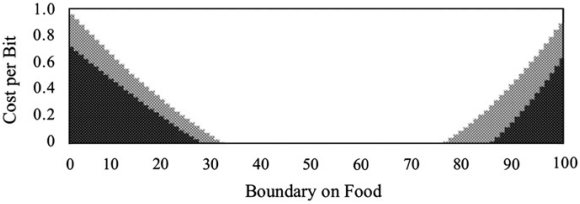
\includegraphics[width=13cm]{Bilder/Single_Resource_Game.png}
  \caption{Genau wahrnehmende Agenten gegen ungenau wahrnehmende}
  \label{fig:sr_game}
\end{center}\end{figure}

Die genauere Wahrnehmung gibt es nicht umsonst. Jedes zusätzliche Bit an Information kostet Energie und Zeit. Die genau wahrnehmenden Agenten entscheiden sich erst für ein Territorium, wenn sie genau wissen, wieviel Futter - der Wertebereich ist 0..100 - darin ist. Die ungenauen Agenten entscheiden aufgrund eines Schwellwerts (boundary) zunächst, ob das Territorium eines mit viel oder wenig Futter ist, und sich dann für das Territorium mit dem vielen Futter. Die grauen Parameterbereiche bedeuten eine Koexistenz beider Arten. In den schwarzen Bereichen überleben nur die genau wahrnehmenden Agenten, im weißen nur die ungenau wahrnehmenden. Haben die ungenau wahrnehmenden Agenten nur einen halbwegs vernünftigen Schwellwert, dann verdrängen sie die genauen Agenten sogar unabhängig von den Informationskosten.

Ein anderes interessantes Ergebnis, das zeigt, wie wir ticken, wird durch Agenten mit mehr und mehr Kategorien, also nicht nur zweien, erhalten. 
\begin{figure}[!h]\begin{center}
  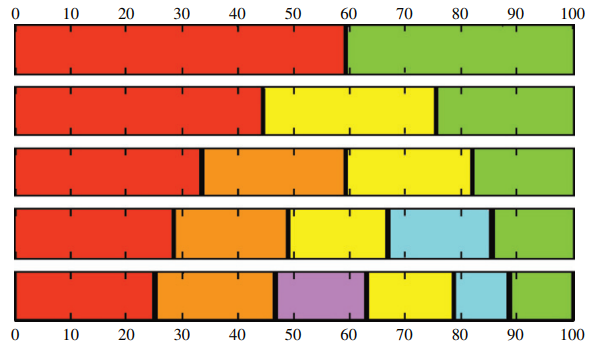
\includegraphics[width=13cm]{Bilder/nCat_Agenten.png}
  \caption{Optimale Postition der Schwellwerte bei verschiedener Anzahl an Kategorien}
  \label{fig:ncat_agents}
\end{center}\end{figure}
Es ist günstig, die Dinge dort genauer zu wissen, wo es etwas zu holen gibt. Wo es nichts zu holen gibt, da haben wir weniger Kategorien. Man könnte es überspitzt auch so sagen: wir haben keine Wörter für Dinge, die es vielleicht geben mag, die uns aber im Hinblick auf unser Überleben nicht interessieren.

\chapter{Einige Begriffe}

\section{Nachricht und Information}

Richtig schwierig ist es, eine vernünftige Definition für den Begriff "Information" zu recherchieren. Auch Wikipedia redet sich im Jahr 2019 hinaus unter Verwendung von Begriffen wie "Wissen", "Signal" und "Code", wodurch nichts erklärt wird. 

Der Physiker Anton Zeilinger sagt über Information:
\begin{quote}\begin{tcolorbox}
Ich bin überzeugt, dass Information das fundamentale Konzept unserer Welt ist. Sie bestimmt, was gesagt werden kann, aber auch, was Wirklichkeit sein kann. In der üblichen Auffassung des Physikers und im täglichen Leben existiert die Wirklichkeit da draußen primär; durch diese Wirklichkeit spazieren wir wie über eine Bühne, und die Information, die wir darüber haben, ist ein sekundäres Konzept. In der Quantenphysik – zumindest in bestimmten Situationen – ist nach meiner Überzeugung die Information das Primäre: das, was gesagt werden kann.
\end{tcolorbox}\end{quote}

Ein fundamentales Konzept unserer Welt ist aus philosophischer Sicht höchst wichtig und wir sollten für den entsprechenden Begriff eine klare Vorstellung entwickeln.

Dazu brauchen wir zunächst die Begriffe "Sender", "Nachricht", "Empfänger": 

\textbf{"Sender", "Nachricht", "Empfänger" sind Teile der Welt, die von uns so bezeichnet werden und an einem Prozess in der Zeit teilnehmen.} 

Dies setzt voraus, dass die Welt in Teile teilbar ist, und das ist eigentlich nie der Fall. Wir kommen darauf noch zurück...

In der Alltagsvorstellung erzeugt ein Sender eine Nachricht dadurch dass er ein Stück Materie oder Energie formt und Richtung Empfänger absendet. Der Empfänger empfängt die Energiematerie und "liest" ihre Geformtheit.

\begin{equation} 
\text{Sender}  \xrightarrow[]{\text{Nachricht}} \text{Empfänger} 
\label{eq:messaging_classical}
\end{equation}

\textbf{Der Informationsgehalt einer Nachricht ist durch die Anzahl N der verschiedenen Veränderungen bestimmt, die sie maximal in irgendeinem Empfänger bewirken kann.} 

Nach der Informationstheorie von C. E. Shannon ist der Informationsgehalt I einer Nachricht über das Eintreffen einer von N möglichen Alternativen
\begin{equation} 
I = \log_2 N 
\end{equation}
und wird in der Einheit \emph{Bit} gemessen.

Beispiel: Wenn nur die Auswahl einer einzigen Farbe aus den Farben {rot, grün, gelb, blau} möglich ist, hat man 4 Alternativen. Um eine Mitteilung über die ausgewählte Farbe zu kodieren sind 2 Bit notwendig. Die Information I ist allgemein eine positive reelle Zahl, denn die Anzahl der Alternativen muss keine Zweierpotenz sein.

Trifft eine Nachricht auf einen ganz simplen Emfänger, der nur 2 Zustände einnehmen kann, so kann ihr wahrer Informationsgehalt höher sein als $\log_2 2 = 1$ aber verborgen bleiben. Der ganze Informationsgehalt kann sich erst mit Empfängern zeigen, die genügend komplex sind.

Der Prozess der Nachrichtenübertragung stellt sich in der Physik so dar:

\begin{equation} 
\begin{split}
\ket{\text{Sendernachricht}} \otimes \ket{\text{Empfänger}} \longrightarrow \\
\ket{\text{Sender}} \otimes \ket{\text{Nachricht}} \otimes \ket{\text{Empfänger}} \longrightarrow \\
\ket{\text{Sender}} \otimes \ket{\text{Nachrichtempfänger}} 
\label{eq:messaging_qm}
\end{split}
\end{equation}

Aus einem Vektor, der oben mit $\ket{\text{Sendernachricht}}$ bezeichnet ist, um damit den Produktraum deutlich werden zu lassen, entschränkt sich ein Vektor und wird dadurch zur Nachricht. Diese Nachricht verschränkt sich mit einem anderen Vektor und beide bilden am Ende einen neuen Vektor, der hier mit Nachrichtempfänger bezeichnet ist. Nur in der Mitte des Prozesses existieren überhaupt Sender, Nachricht und Empfänger. Wir werden auf das Konzept des Produktraums noch zurückkommen...

Mit dieser Darstellung der Nachrichtenübertragung dürfte der Mainstream der Physikergemeinde im Jahr 2019 zufrieden sein. \emph{Doch die Sache hat einen Haken!} Verschränkung ist subjektiv, und damit hängt es von der Sicht auf das Geschehen ab, ob zum Beispiel in der Mitte des Prozesses tatsächlich ein Produktvektor aus 3 Vektoren vorliegt oder nicht. Auch darauf werden wir noch zurückkommen...

Doch das ist nicht das einzige Problem auf dem Weg zur Information als "fundamentalem Konzept unserer Welt". Wir haben postuliert, dass es möglich sein soll, Teile der Welt abzuspalten, die \emph{abzählbar endlich} viele Bits enthalten. \emph{Das steht in krassem Widerspruch zur Vorstellung von kontiunierlichen Empfindungen!} Jede kontinuierliche Variable kann \emph{unendlich} viel Information transportieren. 

Also hat Zeilinger unrecht? Ist Information nur ein kulturelles Konzept? Weil wir langwierig, nicht zuletzt in der Schule, gelernt haben, ein Kontinuum von Empfindungen in endlich viele Schubladen einzusortieren? Oder hat er recht, und das Kontimuum ist gar keines? Raum und Zeit, Impuls und Energie sind nicht kontinuierlich?

\section{Bedeutung}

Genauso schwierig wie für die Information ist es, eine vernünftige Definition für den Begriff "Bedeutung" zu recherchieren. Wikipedia redet sich im Jahr 2019 hinaus unter Verwendung von Begriffen wie "Wissenzusammenhang" und "Sinn", wodurch wieder nichts erklärt wird. 

Wir versuchen es mit folgender einfachen Definition:

\emph{Bedeutung} ist die Änderung, die der Empfang einer Nachricht in einem bestimmten Empfänger auslöst. 

Diese Definition passt zur Alltagsvorstellung der Nachrichtenübertragung gemäß \eqref{eq:messaging_classical}. Obwohl wir nicht bei dieser Definition bleiben werden, liefert sie uns ein sehr wichtiges Ergebnis: \textbf{eine Nachricht enthält niemals Bedeutung}, denn ohne Empfänger gibt es keine Bedeutung. So hat auch diese Schrift keine Bedeutung, ohne dass sie jemand liest.

Da du aufmerksam gelesen hast, wirst du einwenden, dass die unabhängige Existenz des Empfängers mit der Verschränkung mit der Nachricht gemäß \eqref{eq:messaging_qm} endet. Wie können wir da noch von einer nur auf den Empfänger bezogenen Änderung reden? Wir können es nicht!

Der nächste Versuch: 

\textbf{\emph{Bedeutung} ist die Verschränkung, die sich zwischen Nachricht und Empfänger aufbaut, und zwar bei der Zweiteilung ihres gemeinsamen Produktraums unter der Sicht, unter der sie anfangs entschränkt erschienen.}

Da Verschränkung subjektiv ist, müssen wir die Sicht auf das Geschehen mit festlegen, und das haben wir mit dieser Definition getan. Die Sicht ist genau diejenige, die die in  \eqref{eq:messaging_qm} gezeigten Verschränkungen zeigt.

Unabhängig von der weit verbreiteten materialistischen Vorstellung, dass ohne bewusstes Zutun ein objektives Geschehen abläuft, von dem hin und wieder Teile bewusst werden, beharren wir auf einem idealistisch-kritischen Standpunkt: So lange eine Änderung niemandem bewusst wird, so lange muss sie nicht existieren! Bis zur Bewusstwerdung wird es immer eine Glaubensfrage bleiben, ob sich im physikalischen Kanal etwas verändert hat oder nicht. 

Wir gehen nochmal zurück zur Alltagsvorstellung des Nachrichtenübertragungsprozesses \eqref{eq:messaging_classical}. Ein Kranker, der Sender, sendet eine Nachricht, einen hochansteckenden Noro-Virus, an einen Empfänger, einen Gesunden. Welche Bedeutung hat diese Nachricht für den Empfänger?

Wenn wir den Gesunden direkt nach dem Empfang des Noro-Virus fragen, wie es ihm geht, wird er sagen: "wie immer gut". Ein Außenstehender, ein versuchsbegleitender Arzt, wird den Empfänger dagegen als infiziert einstufen. Um die Aussage des Empfängers mit dessem tatsächlichen Zustand in Einklang bringen zu können, entwickelt er das Modell

\begin{equation} 
\text{Empfänger} = \text{Leib} + \text{Bewusstsein}
\end{equation} 

und erzeugt damit das \textbf{Leib-Seele-Problem}: der Leib soll materiell sein und Veränderung nicht bewusst wahrnehmen, während der Arzt mit dem Bewusstsein des Empfängers sprechen kann und sehen kann, dass die Änderung am Leib noch nicht dort angekommen ist. Doch wie funktioniert dann die Kommunikation des Leibes mit dem Bewusstsein, die Kommunikation zwischen Geist und Materie? Wissenschaftliche Ansätze, die auf diesem Modell basieren, können diese Frage im Jahr 2019 nicht beantworten. \emph{Nicht einmal ansatzweise ist eine Lösung des Leib-Seele-Problems auf diesem Pfad erkennbar}.

Was ändert sich, wenn wir auf das physikalische Nachrichtenübertragungsmodell \eqref{eq:messaging_qm} wechseln? Kann damit das Leib-Seele-Problem gelöst werden oder wird alles nur noch schlimmer? Darauf werden wir noch zurückkommen mit Hilfe von Heisenbergs Kette und Wigners Freund...

\section{Nichtkopierbarkeit von Information}

\textbf{Physikalische Information kann im Allgemeinen nicht kopiert werden.}

Es soll also nicht möglich sein, 1 Nachricht zu empfangen, sie zu lesen, und weiterzuschicken? Es soll nicht möglich sein, eine Datei zu kopieren? Jawoll, genau das ist hier die Aussage. Und sie ist wahr. 

Es geht um physikalische Nachrichten. Natürlich ist es schwer, ein Gemälde von Renoir zu kopieren. In der Alltagsvorstellung ist es zumindest denkbar, dass bei perfekter Technik eine perfekte Kopie prinzipiell gelingen kann. Oder bei genügend vielen Versuchen kann zufällig eine exakte Kopie mit abfallen. Die Physik sagt: nein!

Das \textbf{No-Cloning-Theorem} besagt, dass ein Kopierverfahren zwar einzelne Vektoren exakt kopieren kann, aber nur solche, die orthogonal zueinander sind. Nun gibt es immer unendlich viele Linearkombinationen, die neue Vektoren hervorbringen, welche nicht orthogonal zu den anderen sind. Die Wahscheinlichkeit, bei gegebenem Kopierverfahren auf einen Vektor zu treffen, der exakt kopiert werden kann, ist deswegen 0.

Die Unendlichkeit hat nun einen zweites Mal zugeschlagen. Selbst wenn wir nur endlich viel Information in einer physikalischen Nachricht hätten, und sei es nur ein einziges Qubit, aus dem sich maximal ein klassisches Bit auslesen lässt, könnten wir sie mit an Sicherheit grenzender Wahrscheinlichkeit nicht exakt kopieren. 

Aufgrund kultureller Übereinkunft tun wir gemeinsam so tun, als seien ungleiche Empfindungen durch in Wirklichkeit gleiche Dinge verursacht. 

So sagt Chang Tun-Sun

\begin{quote}\begin{tcolorbox}
Wie wir vorstehend gesehen haben, ist die westliche Logik im wesentlichen auf das Gesetz der Identität begründet. Auf ihr beruhen Einteilung, Definition, Syllogismus (Vernunftschluss) und sogar Umkehrung und Widerspruch. Alle diese Begriffe stehen miteinander in Beziehung und bilden ein System.
Die grundlegende Struktur des Chinesischen unterscheidet sich von diesem System. Das chinesische System der Logik, wenn wir es überhaupt ein System nennen wollen, beruht nicht auf dem Gesetz der Identität.
\end{tcolorbox}\end{quote}

und Dürr

\begin{quote}\begin{tcolorbox}
Da wir die Zeit nicht anhalten und zwei Gegenstände nie völlig gleich machen können (zu gleicher Zeit unterscheiden sie sich mindestens durch die Lage), ist es von vornherein gar nicht klar, ob man je die Möglichkeit hat, zweimal „denselben“ Vorgang oder „den gleichen“ Gegenstand zu beobachten. Daß es überhaupt so etwas wie Wiederholbarkeit von Beobachtungen gibt, liegt daran, daß man als Voraussetzung nicht die vollständige Wiederherstellung einer bestimmten Situation fordern muß, sondern nur eine Situation wieder vorbereiten muß, in der alle die für die Beobachtung charakteristischen Merkmale dieselben sind.
\end{tcolorbox}\end{quote}

In unserem Denken gibt es gleiche und ungleiche Dinge, und damit das funktionieren kann muss es unerlaubte Dinge geben, die in der Technik als Sicherheits- oder Störabstand oder dergleichen bezeichnet werden.

Am Beispiel der sogenannten Transistor-Transistor-Logik (TTL) mit 5 Volt Betriebsspannung liest sich dies in Wikipedia so:
"Die Schaltkreise sind so dimensioniert, dass Eingangsspannungen $U_E < 0,8 V$ als Low-Pegel, und $U_E > 2,0 V$ als High-Pegel erkannt werden.
Die Ausgangsspannung $U_A$ beträgt typisch $< 0,4 V$ für den Low-Pegel und $> 2,4 V$ für den High-Pegel bei der zulässigen Last.
Der statische Störabstand beträgt somit sowohl für High- als auch für Low-Pegel $0,4 V$."

\begin{figure}[!h]\begin{center}
  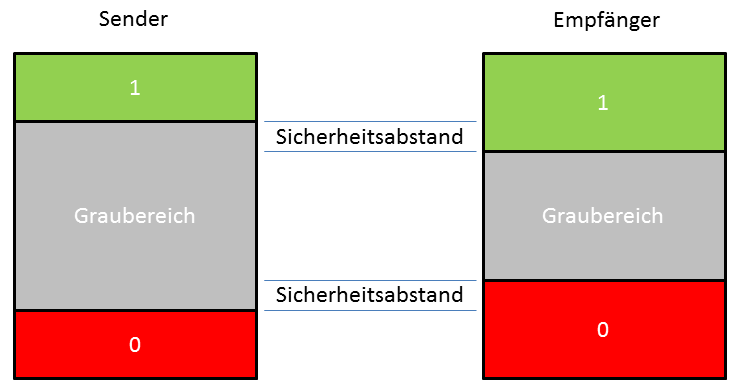
\includegraphics[width=13cm]{Bilder/KlassischesBit.png}
  \caption{Wertebereiche für ein versendetes Bit}
  \label{fig:classical_bit}
\end{center}\end{figure}

Der Empfänger muss eine andere Auffassung davon haben, was 0 und 1 ist, als der Sender, damit Information aus beider Sicht höchstwahrscheinlich kopierbar werden kann. Um auf das Kopieren von Dateien zurückzukommen: selbst wenn die Kopie auf derselben magnetischen Festplatte landen sollte, wird das Magnetfeld anders sein, wenn man nur genau genug hinsieht. Beim Schreiben sind die Feldstärken am Schreiblesekopf viel höher als beim Auslesen. Ganz zu Schweigen davon, dass "die vollkommen gleiche Datei" auf einer DVD vollkommen anders realisiert ist. 

Nur durch kulturelle Übereinkunft gelangen wir zu Nachrichten mit definiertem Informationsgehalt. Wie soll Information ein wesentliches Konzept dieser Welt sein, wenn Menschen zu ihrer Entstehung notwendig sind? Ist Zeilinger noch zu retten? 

\section{Komplexität}

Der Hirnforscher Wolf Singer hat das Gehirn mit seinen rund 500 Billionen Verkehrsknotenpunkten als "die komplexeste Materie des Universums" bezeichnet. 
%https://hpd.de/artikel/woche-steht-im-zeichen-des-gehirns-14187
%https://www.haufe.de/finance/finance-office-professional/von-der-komplexitaet-zur-einfachheit-komplexitaet-verste-11-definition-was-ist-komplexitaet_idesk_PI11525_HI5145449.html
Und der Haufe-Verlag legt nach, denn er weiß, dass "Komplexität heißt: viele Elemente und viele Verbindungen". Damit hat er auch gleich die Ontologie geklärt: alles besteht aus Elementen und Verbindungen. In diesem Abschnitt geht es darum zu zeigen, dass solcherlei Gefasel völliger Quatsch ist.

Um über viel oder wenig reden zu können, braucht man ein \emph{Maß}. Wir brauchen also ein Maß für Komplexität. Tatsächlich gibt es in der Informatik wohldefinierte Komplexitätsmetriken.
%https://de.wikipedia.org/wiki/Komplexit%C3%A4t_(Informatik)
In der Informationstheorie versteht man unter der Komplexität von Daten bzw. einer Nachricht ihren Informationsgehalt, also die Anzahl der Bits. Es gibt alternative Maße wie die Kolmogorow-Komplexität, die den Informationsgehalt als die Größe (für uns idealerweise wieder in Bits gemessen) des kleinsten Programms definiert, das in der Lage ist, die betrachteten Daten zu erzeugen. Bei unendlicher Laufzeit kann ein solches Programm unendlich komplexe Nachrichten erzeugen. Dagegen betrachtet Algorithmische Tiefe die Zeitkomplexität eines optimalen Algorithmus zur Erzeugung der Daten als Maß für den Informationsgehalt.

Wie wir noch sehen werden, hängt eine Nachricht im physikalischen Kanal, die man zum Beispiel als $\psi(x,t)$ schreiben könnte, nach heutiger Vorstellung praktisch immer von kontinuierlichen Variablen, hier $x$ und $t$ für Position und Zeit, ab. Die Mächtigkeit (oder Kardinalität) dieser Nachrichtenmenge wird in der Mathematik als Kardinalität des Kontinuums $|\mathbb{R}|$ bezeichnet. Vollkommen uneingängig mag erscheinen, dass eine endliche Strecke dieselbe Mächtigkeit besitzt wie eine unendliche Fläche oder ein unendlicher fünfzigmilliardendimensionaler kontinuierlicher Raum, aber genau so ist es. Aber die Kardinalität des Kontinuums ist größer als die unendliche Anzahl von natürlichen Zahlen $|\mathbb{R}| > |\mathbb{N}|$. Jegliches Maß, das auf Abzählbarkeit beruht, ist dem Kontinuum nicht angemessen!

Hinzu kommt, dass wir auch die psyische Zeit bislang als kontinuierlich angenommen haben. Damit hat jedes Geschehen automatisch die "Verhaltens"-Komplexität des Kontinuums.

Wir halten also fest:

\textbf{Nach dem bisher Gesagten müssen wir annehmen, dass ein Gehirn genau gleich komplex ist wie ein Stein, und das vollkommen unabhängig von beider Größen. Auch ihr Verhalten müssen wir als gleich komplex ansehen.} 

Die ungleiche Komplexität entsteht durch reduktionistische Schritte, nach denen wir ein komplexeres Modell des Gehirns, wie wir es uns vorstellen, mit einem einfacheren Modell eines Steines, wie wir ihn uns vorstellen, vergleichen. Die unterschiedlichen Komplexitäten in der Vorstellung entstehen durch unterschiedliche Reduktionsschritte, die wir auf beides anwenden. Der Grund, warum wir das unterschiedlich tun, findet sich im Kapitel über die Schleier. 

\section{Gut und Böse}

Im letzten Abschnitt haben wir uns mit den Begriffen "Information" und "Bedeutung" auseinandergesetzt. Bisher haben wir nur wenige Dinge als seiend anerkannt: Empfindungen, Gefühle, Wille und Bewusstsein. Den Informationsbegriff konnten wir nicht abschließend klären, er scheint etwas mit dem physikalischen Kanal zu tun zu haben, das wir noch nicht  verstehen. Am Ende geht es um Veränderung von etwas anerkannt Seiendem, um Veränderung des Bewusstseins, oder um "Bewusstwerden".

Die Wortsprache verwendet sehr viele Begriffe. Wenn diese nichts mit dem zu tun haben, was wir als seiend aufgezählt haben, dann können sie höchstens aus dem stammen, was wir "physikalischer Kanal" genannt haben. Wie wir noch sehen werden, tummeln sich im physikalischen Kanal nach heutiger wissenschaftlicher Auffassung ebenfalls nur wenige Dinge. Demnach müssten sich alle Begriffe auf einige wenige zurückführen lassen.

Wiktionary hilft uns nur ein wenig weiter:
\begin{quote}\begin{tcolorbox}
gut: vom Menschen her positiv bewertet, empfunden, gefühlt und dergleichen

böse: moralisch falsch, nicht gut; bösartig
\end{tcolorbox}\end{quote}

Auf deutsch
\begin{quote}\begin{tcolorbox}
gut: vom Menschen her gut bewertet, empfunden, gefühlt und dergleichen

böse: moralisch böse, nicht gut; bösartig
\end{tcolorbox}\end{quote}
sehen wir die Tautologie und gewinnen nur "vom Menschen her". Menschen haben wir noch nicht als seiend anerkannt, doch wir könnten statt dessen sagen "vom geistigen Seienden  (dem Bewusstsein und Willen) her", und das ist das Einzige, was wir hieraus lernen können. 

Glücklicherweise hat Schopenhauer hier etwas klarer gesehen:
\begin{quote}\begin{tcolorbox}
Ich will aber zuvörderst jene Begriffe gut und böse, welche von den philosophischen Schriftstellern unserer Tage, höchst wunderlicherweise, als einfache, also keiner Analyse fähige Begriffe behandelt werden, auf ihre eigentliche Bedeutung zurückführen; damit man nicht etwan in einem undeutlichen Wahn befangen bleibe, daß sie mehr enthalten, als wirklich der Fall ist, und an und für sich schon alles hier Nöthige besagten ...
Also Alles, was dem Willen in irgend einer seiner Aeußerungen zusagt, seinen Zweck erfüllt, das wird durch den Begriff gut gedacht, so verschieden es auch im Uebrigen seyn mag. Darum sagen wir gutes Essen, gute Wege, gutes Wetter, gute Waffen, gute Vorbedeutung u.s.w., kurz, nennen alles gut, was gerade so ist, wie wir es eben wollen; daher auch dem Einen gut seyn kann, was dem Andern gerade das Gegentheil davon ist ...
Der Begriff des Gegentheils wird, so lange von nichterkennenden Wesen die Rede ist, durch das Wort schlecht, seltener und abstrakter durch Uebel ausgedrückt, welches also alles dem jedesmaligen Streben des Willens nicht Zusagende bezeichnet. Wie alle andern Wesen, die in Beziehung zum Willen treten können, hat man nun auch Menschen, die den gerade gewollten Zwecken günstig, förderlich, befreundet waren, gut genannt, in der selben Bedeutung und immer mit Beibehaltung des Relativen, welches sich z.B. in der Redensart zeigt: »Dieser ist mir gut, dir aber nicht.« Diejenigen aber, deren Charakter es mit sich brachte, überhaupt die fremden Willensbestrebungen als solche nicht zu hindern, vielmehr zu befördern, die also durchgängig hülfreich, wohlwollend, freundlich, wohlthätig waren, sind, wegen dieser Relation ihrer Handlungsweise zum Willen Anderer überhaupt, gute Menschen genannt worden. Den entgegengesetzten Begriff bezeichnet man im Deutschen und seit etwan hundert Jahren auch im Französischen, bei erkennenden Wesen (Thieren und Menschen) durch ein anderes Wort als bei erkenntnißlosen, nämlich durch böse, méchant, während in fast allen andern Sprachen dieser Unterschied nicht Statt findet und kakos, malus, cattivo, bad von Menschen wie von leblosen Dingen gebraucht werden, welche den Zwecken eines bestimmten individuellen Willens entgegen sind.
\end{tcolorbox}\end{quote}
%[Schopenhauer-D 1. Band §65]

\textbf{Gut und böse sind nichts weiter als Synonyme für das, was der Wille will beziehungsweise nicht will. Wenn es verschiedene Willen mit verschiedenen Richtungen gibt, gibt es kein absolut Gutes und kein absolut Böses.}

\section{Sinn}

Als sinnvoll wird etwas bezeichnet, was die Wahrscheinlichkeit für die Erreichung eines Ziels, berechnet nach einem Ursache-Wirkungsmodell, erhöht. Mit Ursache und Wirkung müssen wir uns noch genauer beschäftigen. Das Ziel, das heißt gewollte Empfindungen, ist immer irgendwie zufällig. Die Frage nach dem Sinn des Lebens ist die Frage nach einem absoluten Sinn. Einen solchen absoluten Sinn kann es nur geben
\begin{itemize}
\item im Solipsismus. Dann ist der Sinn die Erfüllung des \emph{einen} Willens.
\item im Nicht-Solipsismus nur, wenn alle Willensrichtungen in Übereinstimmung gebracht werden können.
\end{itemize}
Den Solipsismus hat diese Schrift bereits ausgeklammert. Bei Existenz mehrerer Bewusstseine hieße die Übereinstimmung derer Willensrichtungen, dass die Ziele aller auch von allen gewollt sind. Etwas schwächer ausgedrückt sollten die Ziele aller von allen mindestens als neutral empfunden werden, nicht jedoch als schlecht. Je mehr Bewusstseine es gibt, desto unwahrscheinlicher wird dieser Fall. Die Wahrscheinlichkeit für einen absoluten Sinn hängt also an der Anzahl der Bewusstseine, und wie wir noch sehen werden, muss die Zahl die Antwort auf eine Glaubensfrage bleiben, so lange es einen physikalischen Kanal zwischen Bewusstseinen gibt. Es gibt jedoch Gründe, an sehr viele Bewusstseine zu glauben, wodurch die Wahrscheinlichkeit dafür, dass des einen Freude des anderen Leid bedeuten würde, gegen 1 ginge. In diesem Fall könnte die Frage nach dem absoluten Sinn des Lebens klar beantwortet werden: es gibt keinen! Man könnte auch sagen: Gott denkt so nicht! Heraklit hat es diese Erkenntnis so ausgedrückt: 
\begin{quote}\begin{tcolorbox}
Für Gott ist alles schön und gut und recht; nur die Menschen sind der Meinung, das eine sei recht, das andere unrecht.
\end{tcolorbox}\end{quote}

\subsection{Theodizee}

"Wie kann ein gütiger allmächtiger Gott zulassen, dass so viel Leidvolles in der Welt geschieht?" Gibt es tatsächlich viele Bewusstseine, deren Willensrichtungen natürlicherweise nicht übereinstimmen bzw. entgegengesetzt sind, so ist diese Fragestellung größenwahnsinnig und egozentrisch. Denn:
\begin{itemize}
\item Da "gut" nur ein weiteres Wort für das ist, was ein Wille will, ist ein gütiger Gott einer, der das will, was der, der die Frage gestellt hat, will.
\item "leidvoll" ist nur ein weiteres Wort für das, was ein Wille nicht will, also für das, was der, der die Frage gestellt hat, nicht will.
\end{itemize}

Die Frage meint also eigentlich: "Wie kann jemand Allmächtiges, der immer genau das will, was ich will, zulassen, das soviel geschieht, was ich nicht will?" Oder anders ausgedrückt, da ja jemand, der immer genau das will, was ich will, mit Sicherheit ich selber bin: "Warum eigentlich bin ich nicht selber der allmächtige Gott?" Diese größenwahnsinnige egozentrische Frage ist die Frage der Theodizee. Willst du nun noch auf diese Frage weiterhin nach einer Antwort suchen?

\section{Lebendig und Tot}

Was ist Leben? Wikipedia meint
"Was Leben bzw. ein Lebewesen ist, wird - in der modernen Biologie wie schon bei Aristoteles - nicht über einzelne Eigenschaften, einen bestimmten Zustand oder eine spezifische Stofflichkeit definiert, sondern über eine Menge von Aktivitäten, die zusammengenommen für Leben bzw. Lebewesen charakteristisch und spezifisch sind. Als diese Aktivitäten werden üblicherweise genannt:"
\begin{itemize}
\item "Energie- und Stoffwechsel und damit Wechselwirkung mit ihrer Umwelt."
\item "Organisiertheit und Selbstregulation (Homöostase)."
\item "Reizbarkeit, das heißt sie sind fähig, auf chemische oder physikalische Änderungen in ihrer Umwelt zu reagieren."
\item "Fortpflanzung, das heißt, sie sind zur Reproduktion fähig.
Vererbung, das heißt, sie können Informationen (Erbgut) an ihre Nachkommen übermitteln.
Wachstum und damit die Fähigkeit zur Entwicklung."
\end{itemize}

Mit der Wikipedia-Definition von Leben dürften die meisten Menschen etwas anfangen können. Es gibt jedoch Kunde von einigen sehr intelligenten Herren, die ganz anderer Auffassung waren:

Heraklit:
\begin{quote}\begin{tcolorbox}
Ein und dasselbe ist Lebendiges und Totes und Wachendes und Schlafendes und Junges und Altes; denn dies schlägt um und ist jenes, und jenes wieder schlägt um und ist dies.
\end{tcolorbox}\end{quote}
Heisenberg:
\begin{quote}\begin{tcolorbox}
Im Gebiet der kleinsten Organismen kann ja auch die Frage, ob ein bestimmtes Gebilde ein „lebendes Wesen“ oder ein Stück „toter Materie“ sei, nur durch willkürliche Definitionen beantwortet werden.

Bei diesen kleinsten Lebewesen aber wird die Frage, ob sie aus lebendiger oder toter Materie bestehen, unentscheidbar. Man kann dies so ausdrücken, daß es überhaupt nur lebendige Materie gebe; ...

Gehört die eben aufgenommene Nahrung, die Luft, die eingeatmet wurde, mit zum Körper, oder nicht? Von welchem Zeitpunkt ab sollen sie als Teile des Körpers bezeichnet werden? Gehört das Schneckenhaus mit zum Organismus der Schnecke, das Netz mit zu dem der Spinne? Müsste nicht bis zu einem gewissen Grad auch das Erdreich, in dem die Pflanze wurzelt, mit zu ihrem lebendigen Zusammenhang gerechnet werden?
\end{tcolorbox}\end{quote}

Und Dürr wird hier noch deutlicher:
\begin{quote}\begin{tcolorbox}
Eigentlich gibt es gar nichts Unlebendiges!

Dass ein Tisch im Grunde auch lebendig ist, bemerken wir nicht, weil wir ihn nur vergröbert betrachten und damit vereinfacht sehen.
\end{tcolorbox}\end{quote}

Hier machen wir reinen Tisch, sparen uns dabei vernichtende Kritik an der Wikipedia-Definition, welche sehr leicht zu äußern wäre, und benutzen statt dessen die folgende Abgrenzung:

\textbf{Lebendig ist das Bewusstsein mitsamt all dem, was wir bereits als Seiend und mit jenem im Zusammenhang stehend oder gar in Einheit befindlich erkannt haben: Empfindungen, Gefühle, Wille.} 

\textbf{Tot ist alles andere, also der physikalische Kanal, der sich zwischen dem Lebendigen befindet.}

Wie dünn oder dick dieser physikalische Kanal ist, wissen wir nicht. Wir werden uns aber noch ausführlich mit ihm befassen.

\section{Intelligenz}

Wikipedia sagt: "Intelligenz ist in der Psychologie ein Sammelbegriff für die kognitive Leistungsfähigkeit des Menschen. Da einzelne kognitive Fähigkeiten unterschiedlich stark ausgeprägt sein können und keine Einigkeit besteht, wie diese zu bestimmen und zu unterscheiden sind, gibt es keine allgemeingültige Definition der Intelligenz. Vielmehr schlagen die verschiedenen Intelligenztheorien unterschiedliche Operationalisierungen des alltagssprachlichen Begriffs vor."

Wieder können wir mit dieser Definition nichts anfangen, da sie auf dem Begriff Mensch aufbaut, und die Existenz von Menschen zweifeln wir nach wie vor an. Würden wie sie nicht anzweifeln, dann würden wir auch an Affen und Vögel glauben und müssten uns wenigstens fragen, warum diese nicht intelligent sein sollten. Es scheint ja auch nicht möglich zu sein, sich im System des naiven Realismus auf eine Definition zu einigen. Damit soll aber ab dieser Stelle genug der Polemik gegen derartiges Schrifttum sein. Die Botschaft, dass selbst auf Konsens basierenden Ergebnissen eines formalisierten Abstimmungsprozesses nicht zu trauen ist, ist hoffentlich bei dir angekommen. Denke selbst! 

\textbf{Intelligenz} misst, wie stark ein Wille die Wahrscheinlichkeit für zukünftigen Schmerz verringern und für zukünftige Lust vergrößern kann aufgrund gespeicherter Information aus vergangenen Empfindungen unter Zuhilfenahme eines Verstandes/Gehirns/Rechenwerks.

In dieser Definition haben wir Rückgriff genommen auf den \emph{Willen}, \emph{Empfindungen}, \emph{Gefühle}, \emph{Information} und die \emph{psychische Zeit}. Wir haben aber zusätzlich postuliert, dass es ein Rechenwerk geben soll, dass aus Informationen Wahrscheinlichkeiten für Empfindungen berechnen kann. Dieses Rechenwerk soll auf einen Speicher zugreifen können, der ein Modell (in psychischer Zeit) vergangener Empfindungen enthält. Auf die Suche danach müssen wir noch gehen, vielleicht finden wir etwas im physikalischen Kanal?

\subsection{Künstliche Intelligenz gibt es nicht}

Um eine künstliche Intelligenz gemäß unserer Definition zu erschaffen, genauer spricht man hierbei von "starker KI", müssten unter anderem künstlich erschaffen werden

\begin{itemize}
\item Wille
\item Schmerz und Lust
\item Psychische Zeit
\end{itemize}

Die Schaffung einer starken KI ist nichts anderes als die Schaffung von Geist, und eben aus diesem Grund wird sie niemals gelingen. So gibt Wikipedia zu:
"Die Ziele der starken KI sind nach Jahrzehnten der Forschung weiterhin visionär." Anders ausgedrück: es ist nichts dabei herausgekommen.

Natürlich kann es sein, dass bei mehr oder weniger blindem Herumgedoktere an Information und Rechenwerken irgendwann zufällig etwas abfällt, das bereits bekanntem Verhalten verblüffend ähnelt. Es kann sogar sein, dass dieses Etwas mit Geist derart verbunden ist, dass es unsere Definition für Intelligenz erfüllt. Dann wird man gerne glauben, man hätte nicht nur die Verbindung zum Geist, sondern den Geist gleich mit erschaffen. Darauf, ob wir überhaupt erkennen können, wo außer dem eigenen noch anderer Geist sitzt, werden wir noch zurückkommen.


\chapter{Der physikalische Kanal}
Wir sehen uns zunächst eine Aussage Wolfgang Paulis aus einem unpublizierten Aufsatz vom Juni 1948 an.
% Appendix 3 Wolfgang Pauli und C. G. Jung, Ein Briefwechsel 1932-1958, Springer-Verlag
\begin{quote}\begin{tcolorbox}
Gemäß ihrer Definition muss die Physik das Gesetzmäßige in der Natur begrifflich darstellen und hat deshalb ihre Aufmerksamkeit nur auf das Reproduzierbare und auf das quantitativ Messbare zu richten. Als Folge dieser im Wesen der Physik liegenden Beschränkung bleibt nicht nur alles Gefühlsmässige, Wertende und Emotionale ausserhalb ihrer auf der psychologischen Gegenseite, sondern aus dieser Wurzel entspringt auch der statistische Charakter ihrer Aussagen, der insbesondere bei den atomaren Vorgängen auf die Erfassung des Einzelfalles (abgesehen von Spezialfällen) grundsätzlich verzichten muss. Hierbei handelt es sich aber nicht um eine Unvollständigkeit der Quantentheorie innerhalb der Physik, sondern um eine Unvollständigkeit der Physik innerhalb des gesamten Lebens.
\end{tcolorbox}\end{quote}
Der Physik-Nobelpreisträger des Jahres 1945 liefert uns hier einen Haufen wertvolle Fingerzeige.

Es soll eine Wissenschaft vom Gesetzmäßigen geben. In der Natur sollen demnach gesetzmäßige Vorgänge ablaufen, und die Wissenschaft davon ist die \emph{Physik}. Anstatt Physik könnte man auch ganz allgemein \emph{Naturwissenschaft} sagen, denn die heutige Naturwissenschaft arbeitet generell nach dieser Methode: quantitative Messungen mit anschließender Gewinnung mathematischer Modelle aus den Messergebnissen.

Außerhalb dieser Physik sieht Pauli all das Geistige, dessen Existenz wir zuallererst anerkannt haben. Pauli sagt deutlich, dass dieses Geistige, dieses Psychische, eben nicht gesetzmäßig funktionieren soll. Das ist höchst erstaunlich, denn woher will er das so genau wissen? Ist der Wille "frei" von Gesetzmäßigkeit? 134 Jahre zuvor noch lehnte sich sein ebenso berühmter Kollege Laplace zusammen mit seinem nach ihm benannten Dämon aus dem Fenster des Essai philosophique sur les probabilités und verkündete das Gegenteil: alles in der Natur laufe gesetzmäßig ab.

Schließlich warnt uns Pauli davor zu glauben, mit der gesetzmäßigen Naturbeschreibung sei die Arbeit getan. Nein, wenn die Naturbeschreibung dabei stehen bleibt, dann wird sie immer unvollständig sein. Die Unvollständigkeit ist nicht eine Unvollständigkeit der Quantentheorie, wie es vielleicht ein Albert Einstein noch hoffen wollte, sondern eine Unvollständigkeit der Physik, ja der gesamten es ihr gleichtuenden modernen Naturwissenschaft. Anfang des 21. Jahrhunderts müssen wir eigentlich nicht mehr zwischen Quantentheorie und dem Rest der Physik unterscheiden. Kaum ein moderner Physiker dürfte noch daran glauben, dass irgendwelche seiner erprobten physikalischen Gesetze auf etwas anderes wie eine Quantentheorie zurückzuführen seien. Daran ändert die Tatsache, dass es noch keine befriedigende Quantentheorie gibt, die die Gravition beschreibt, nichts. Es gibt Quantentheorien für den Grenzfall schwacher Gravitation. Es gibt Kandidaten für Quantengravitationstheorien, die sich der experimentellen Überprüfbarkeit noch entziehen. Es gibt Vorschläge für Experimente, die den Quantencharakter der Gravitation zeigen oder widerlegen können, unabhängig von der konkreten Theorie, mit der sie zu beschreiben wäre. 

Für uns bezeichnet ab sofort \emph{Physik immer dasselbe wie Quantenphysik}. \textbf{Der physikalische Kanal zwischen den Bewusstseinen ist ein Quantenkanal.} Eine große Frage, die uns beschäftigen wird, ist: Wie lang ist er denn, dieser Kanal? Wieviel ist geistig, also lebendig, und wieviel nichtgeistig, also tot? Zunächst müssen wir verstehen, wie der physikalische Kanal aus heutiger Sicht funktioniert...

Noch ein letzter Hinweis: längst nicht alle heutigen Physiker oder Naturwissenschaftler, eher eine Minderheit, werden Pauli darin beipflichten, dass das Geistige außerhalb des Quantengesetzmäßigen zu beschreiben sei. Leute wie Tegmark oder Penrose versuchen sich an einer bisher vergeblichen Erklärung des Geistigen aus dem Physikalischen heraus.

\section{Die Struktur der Quantenmechanik}

\section{Physikalische Zeit}

\chapter{Wie viele?}


\end{document}